\chapter{Evaluation}
\label{sec:evaluation}
Inspired by previous research~\cite{Collberg, Ma, Maieee}, we evaluate our
Turing machine obfuscator based on four metrics which are
\textit{potency}, \textit{resilience}, \textit{stealth} and \textit{cost}
respectively. We also evaluate the functionality correctness of the obfuscated
binaries. Potency weighs the complexity of the obfuscated programs, which is
straightforward to show how competent an obfuscator is. A good obfuscator also
needs to protect itself from being deobfuscated; to measure how well an
obfuscated program is resilient to automatic deobfuscation techniques, we
evaluate the resilience of our Turing machine obfuscator. Moreover, in the
battle against experienced attackers, obfuscated programs should not be too
distinguishable from its origins otherwise it would be easy to be recognized.
Hence, we measure the stealth to show how well an obfuscated program resembles
the original one. Cost is naturally employed to measure the execution overhead
of a software program. While obfuscation would inevitably introduce performance
penalty, we measure the execution time of the obfuscated code to show the
overall cost is acceptable.

Two widely-used open source programs are employed in our evaluation: compress
tool \textsc{bzip2} (version 1.0.6)~\cite{bzip2} and regular expression engine
\textsc{regexp} (version 1.3)~\cite{slre}. Obfuscation level is an index which
represents the ratio between obfuscated instructions and all candidates. In our
experiments, the ratio is set as 50\% which means half of all conditional
transfer candidates are randomly selected and obfuscated.

\section{Functionality}
Both programs evaluated in our research (\textsc{bzip2}~\cite{bzip2} and
\textsc{regexp}~\cite{slre}) provide test cases to verify the functionality of
the compilation outputs. In particular, the \textsc{bzip2} test cases deliver 3
compression samples and 3 decompression samples, while the \textsc{regexp} test
cases contain 149 samples of various regular expression patterns. We leverage
those shipped test cases to verify the functionality correctness of our
obfuscated programs. For all the evaluated obfuscation levels (i.e., 30\%, 50\%,
80\% and 100\%), we report all the obfuscated programs can pass all the test
cases, hence preserving the original semantics after obfuscation.

\section{Potency}
Control flow graph (CFG) and call graph provide insights on the general
structure of a program and they are the foundation for most static software
analysis. With the help of IDA Pro~\cite{ida}, a well-known commercial binary
analysis tool, we recover CFG and call graph information from both original and
obfuscated binaries. By traversing the graph, we further calculate the number of
basic blocks, number of call graph and control graph edges. We use such
information to measure the complexity of a program, which is aligned with
previous research~\cite{Chen}. Analysis result are shown in Table~\ref{tab:two}.
Comparing the original and obfuscated programs, it can be observed that program
complexity is increased in terms of each metric.

\begin{table}
  \centering
 \caption{Potency evaluation in terms of program structure-level information.}
 \label{tab:two}
 \begin{tabular}{|c|c|c|c|}
 \hline 
 \textbf{Program} & \textbf{\# of CFG Edges} & \textbf{\# of Basic Blocks} & \textbf{\# of Function} \\
 \hline
\textsc{bzip2} & 3942 & 2647 & 78 \\ 
 \hline
obfuscated \textsc{bzip2} & 4195 & 2828 & 134 \\
 \hline
\textsc{regexp} & 906 & 619 & 25 \\ 
 \hline
obfuscated \textsc{regexp} & 1122 & 773 & 43 \\
 \hline
\end{tabular}
\end{table}

We further quantify the Turing machine obfuscated programs w.r.t. the cyclomatic
number and knot number (these two metrics are introduced in
\cite{McCabe,Woodward}). Cyclomatic metric is defined as \[ Cyclomatic = E - N +
2 \] where E and N represent the number of edges and the number of nodes in a
CFG, respectively. Knot number shows the number of edge crossings in a CFG.
These two metrics intuitively weigh how complicated a program is in terms of
logic diversion number. Results in Table~\ref{tab:three} shows that both knot
number and cyclomatic number notably increase after Turing machine obfuscation.
Overall, we interpret Table~\ref{tab:two} and Table~\ref{tab:three} as promising
results to show program becomes more complex after the Turing machine
obfuscation.

\begin{table}
  \centering
 \caption{Potency evaluation in terms of knot and cyclomatic number.}
 \label{tab:three}
 \begin{tabular}{|c|c|c|}
 \hline 
 \textbf{Program} & \textbf{\# of Cyclomatic} & \textbf{\# of Knot} \\
 \hline
\textsc{bzip2} & 1297 & 5596  \\ 
 \hline
obfuscated \textsc{bzip2} & 1369 & 5720  \\
 \hline
\textsc{regexp} & 289 & 478 \\ 
 \hline
obfuscated \textsc{regexp} & 351 & 1068 \\
 \hline
\end{tabular}
\end{table}

Besides picking 50\% as the obfuscation level in evaluating potency, we also
conduct experiments with obfuscation levels as 30\%, 80\% and 100\%.
\F~\ref{fig:seven} shows the number of call graph edges regarding different
obfuscation levels. Observation shows that with a higher obfuscation level, the
number of call graph edges increases. We interpret the results that the
obfuscated program become more complicated with the obfuscation level increases.

\begin{figure}
  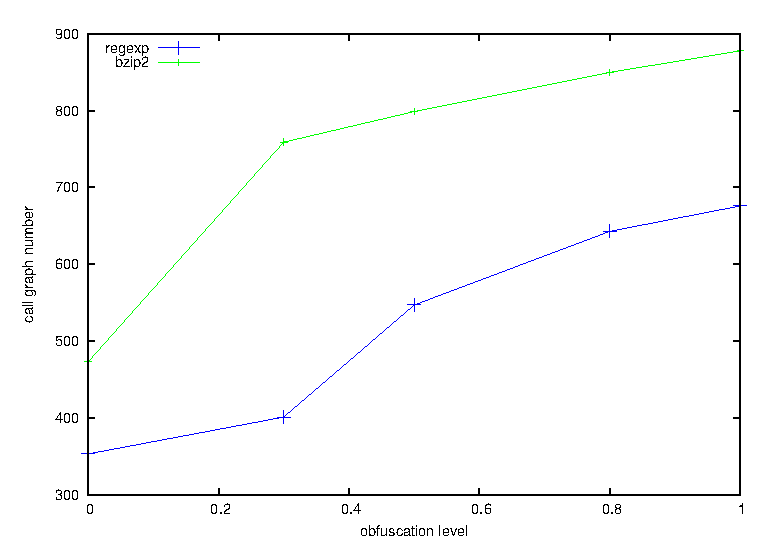
\includegraphics[width=0.9\linewidth]{cg.eps}
  \caption{Number of call graph edges in terms of different obfuscation levels.}
  \label{fig:seven}
\end{figure}

\section{Resilience}
\label{subsec:resilience}
A good obfuscation technique should resist deobfuscation tools as well. Concolic
testing is an advanced deobfuscation technique aiming at finding bugs or
vulnerabilities in software through the mixture of symbolic execution and
concrete execution. Whereas, it is also used by adversaries to analyze or
restore software control flow graph~\cite{Cadar,Sen,Cute}. KLEE~\cite{klee} is a
static analysis tool based on the LLVM platform and it could generate enough
test cases to largely increase the path coverage. With the help of KLEE, it
would be easy to conduct automated deobfuscation by concolic testing. We choose
KLEE as the deobfuscation tool to evaluate resilience of Turing Machine
obfuscator. We used a piece of sample code from KLEE~\cite{kleesample} as the
subject program (the sample code is shown in \F~\ref{fig:klee-sample}). The
subject program need to be converted to IR codes since KLEE works on IR level.

\begin{figure}[h]
\centering
\begin{lstlisting}
    int get_sign(int x) {
      if (x == 0)
        return 0; 

      if (x < 0)
        return -1;
      else 
        return 1;
    }

    int main() {
      int a;
      klee_make_symbolic(&a, sizeof(a), "a");
      return get_sign(a);
    }
\end{lstlisting}
\caption{KLEE sample code used in our evaluation. All the path conditions are obfuscated.}
\label{fig:klee-sample}
\end{figure}


KLEE could detect three paths in the original subject program as expected. Based
on different value of x, this program may traverse branches in which x equals 0,
x is less than 0 and x is greater than 0, respectively. In contrast, after
subject program is obfuscated by our Turing machine obfuscator, we report that
KLEE could only figure out \textbf{one} path. We interpret the evaluation result
that Turing machine obfuscator can impede automated deobfuscation tools from
restoring the structure of a program.

Due to limited information released by KLEE, we could not figure out the
underlying reason that leads to the failure of KLEE. Since Turing machine
obfuscator makes the conditional branches more complicated, we envision that the
internal constraint solver employed by KLEE is unable to yield a proper symbolic
input which ``drill'' into the branches protected by our Turing machine
obfuscator.

\section{Stealth}
As mentioned in the beginning, software obfuscation technique should not only
combat automated deobfuscation tools, but also manual deobfuscation methods. In
the evaluation of stealth, Wang et al.~\cite{Trans} compare the instruction
distributions of the original and obfuscated programs. If instruction
distribution of the obfuscated program is distinguishable from its original
program (e.g., \texttt{call} or \texttt{jmp} instruction proportions are
abnormally high), it would be an indicator that the program is manipulated. We
adopted this metric to evaluate our Turing obfuscator. Obfuscation level for
stealth evaluation is set to 50\%.

\begin{figure}
  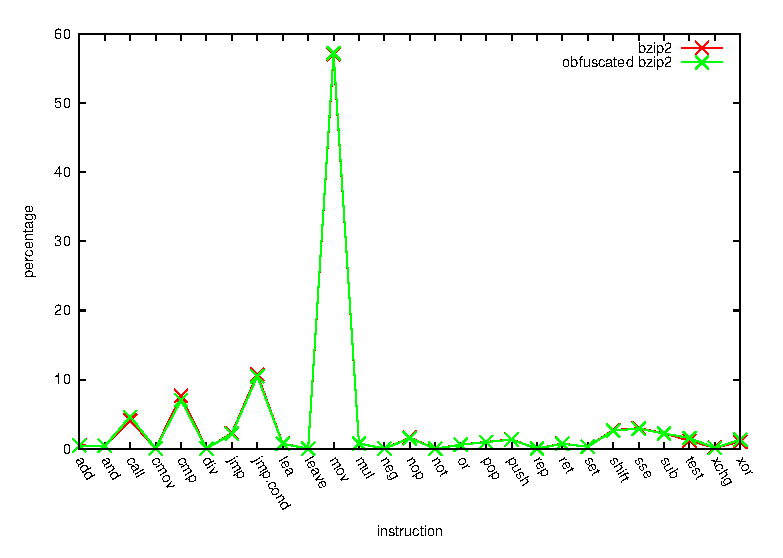
\includegraphics[width=0.9\linewidth]{st_bzip2.eps}
  \caption{\textsc{bzip2} instruction distribution comparison.}
  \label{fig:bzip2}
\end{figure}

\begin{figure}
  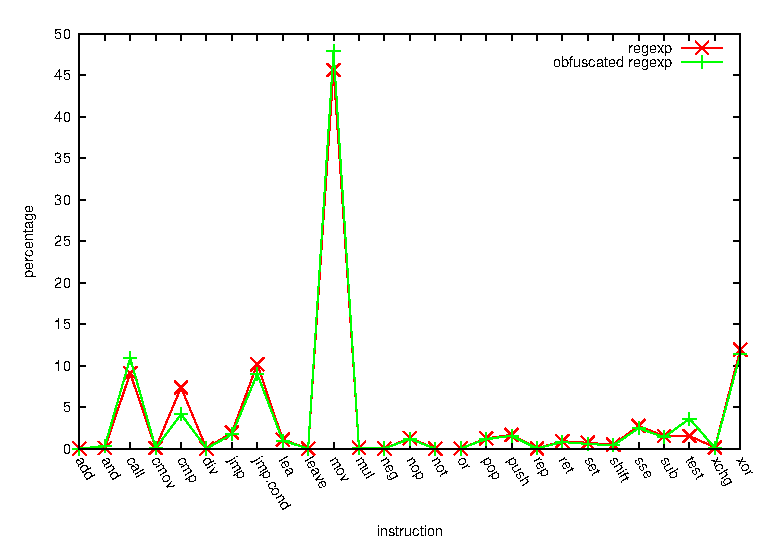
\includegraphics[width=0.9\linewidth]{st_regexp.eps}
  \caption{\textsc{regexp} instruction distribution comparison.}
  \label{fig:regexp}
\end{figure}

Consistent with previous research~\cite{Trans}, we put assembly instructions
into 27 different categories. \F~\ref{fig:bzip2} and \F~\ref{fig:regexp} present
the instruction distribution of the original and obfuscated programs
(\textsc{bzip2} and \textsc{regexp}). Experiment results indicate that the
instruction distribution after obfuscation is very close to the origin
distribution.
%% Moreover, we notice that the instruction distribution variance of
%% \textsc{regexp} is slightly higher than \textsc{bzip2}. This observation makes
%% sense since \textsc{regexp} consists of 8117 lines of C code while
%% \textsc{regexp} contains only 1391 lines of C code.
In sum, small instruction distribution variation is a promising result to show
the proposed technique would obfuscate programs in a stealthy way.

\section{Cost}
Software running cost is another critical factor in evaluating an obfuscation
technique. In most obfuscation research work, execution cost is inevitably
increased because obfuscation would bring in extra instructions. Measuring the
execution time is a convincing way to evaluate to the cost.

In our evaluation, both original and obfuscated programs are executed on a
server with 2 Intel(R) Xeon(R) E5-2690 2.90GHz processors and 128GB system
memory. \textsc{bzip2} is used to compress three different sample files and
regular expression engine \textsc{regexp} runs 149 samples provided in its
shipped test cases. We run each program three times and record the average
time cost as the final result.

\begin{figure}
  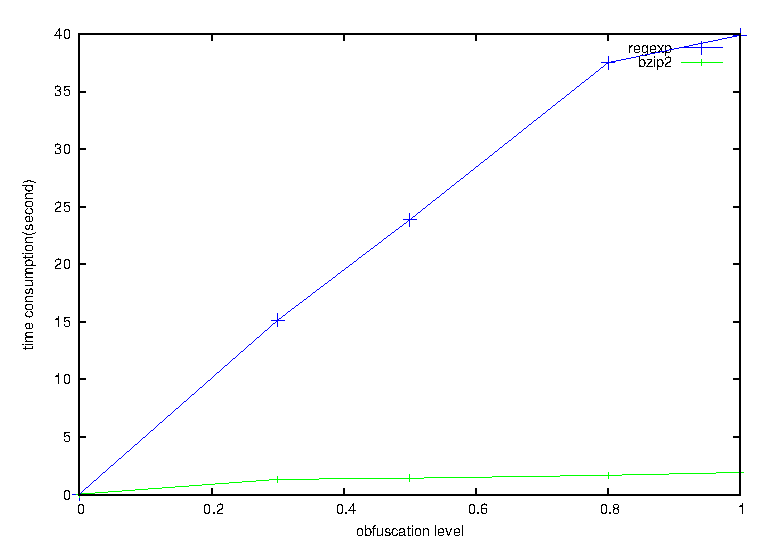
\includegraphics[width=0.9\linewidth]{cost.eps}
  \caption{Execution overhead in terms of different obfuscation levels.}
  \label{fig:cost}
\end{figure}

\F~\ref{fig:cost} shows that for both test cases, the execution slowly grows
w.r.t the increase of obfuscation levels. As expected, program takes more time
to execute with more instructions are obfuscated. On the other hand, we
interpret the overall time cost is still confined to a reasonable level. We also
notice that there exists a difference between slopes of the two curves. Turing
obfuscator randomly obfuscates candidate instructions within the program before
execution. Hence the transformed instructions may not be indeed executed in the
runtime. Difference between two curve slopes is probably due to such uncertainty
of execution. In addition, some further study on the source code show that
\textsc{regexp} employs more recursive calls than \textsc{bzip2}, thus may lead
to more invocations of the Turing machine component and contribute to the
performance penalty.
